The following python codes generate the required circle
	\begin{lstlisting}
	./solutions/5/codes/circle/q18abc.py
	./solutions/5/codes/circle/q18d.py
	\end{lstlisting}


\begin{enumerate}

\item \begin{align} 
\vec{x^Tx} - \myvec{4\\8}\vec{x} -45 = 0
\end{align}
See Fig. \ref{fig:4.2.5_qoeabc}.
\begin{align}
\vec{O} = \myvec{2\\4}, r = \sqrt{65} 
\end{align}
	\begin{figure}[!ht]
	\centering
	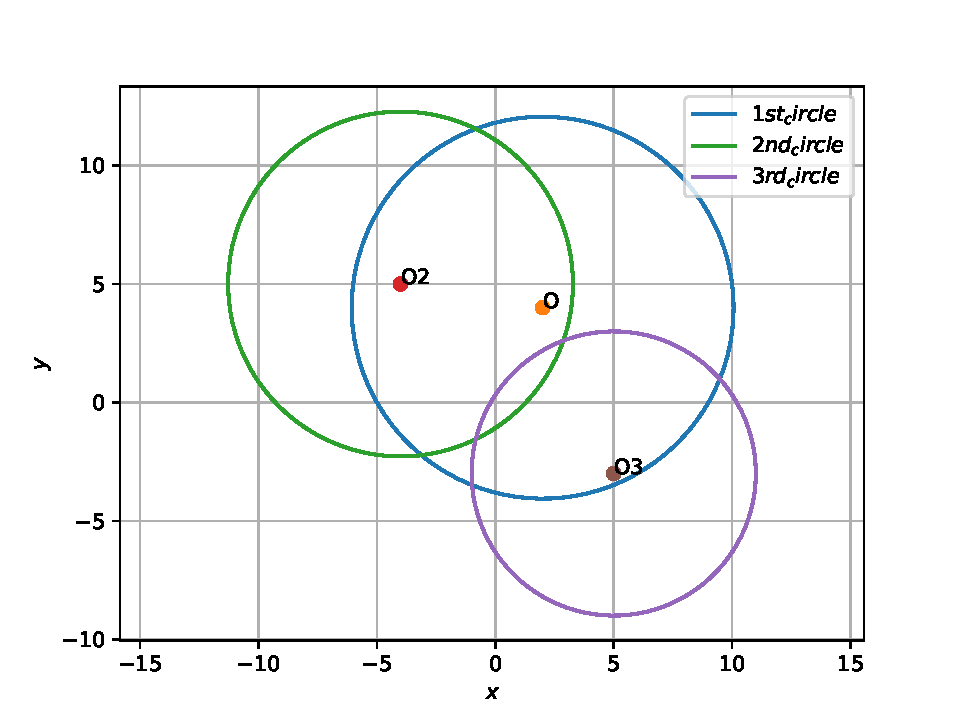
\includegraphics[width=\columnwidth]{./solutions/5/figs/circle/q18abc.eps}
	\caption{}
	\label{fig:4.2.5_qoeabc}	
	\end{figure}

\item See Fig. \ref{fig:4.2.5_qoeabc}.
\begin{align}
\vec{O} = \myvec{-4\\5}, r = \sqrt{53} 
\end{align}

\begin{align} 
\vec{x^Tx} - \myvec{8\\-10}\vec{x} - 12 = 0
\end{align}


\item See Fig. \ref{fig:4.2.5_qoeabc}.
\begin{align}
\vec{O} = \myvec{5\\-3}, r = 6
\end{align}
\begin{align} 
\norm{x - \myvec{5\\-3}} = 36
\end{align}



\begin{comment}
	\begin{figure}[!ht]
	\centering
	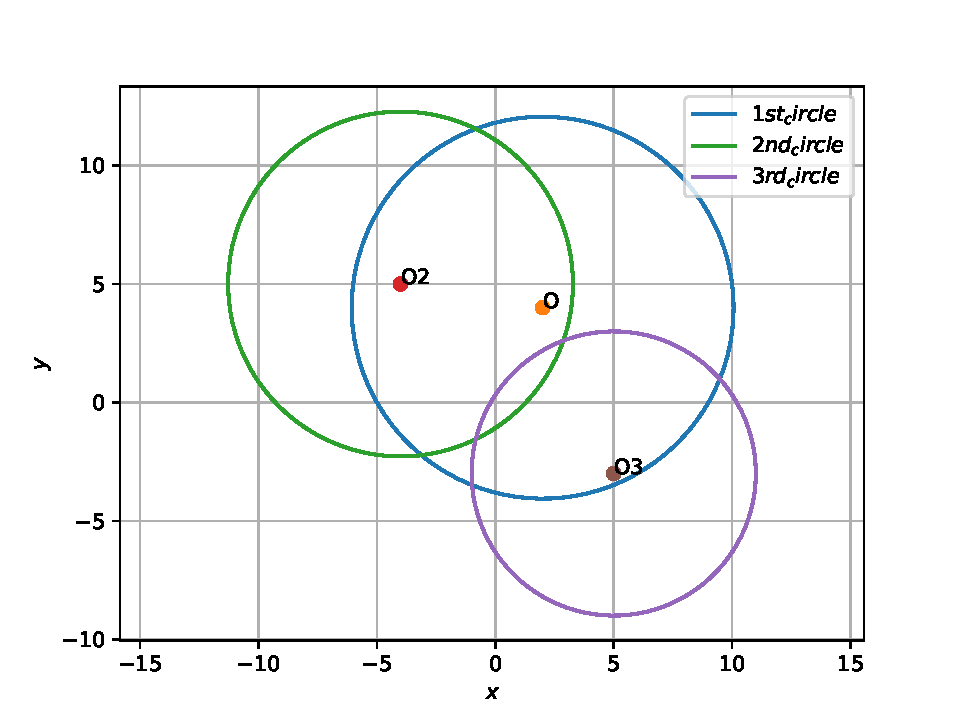
\includegraphics[width=\columnwidth]{./solutions/5/figs/circle/q18abc.eps}
	\caption{Circle of Q.4.2.5}
	\label{fig:4.2.5_qoeb}	
	\end{figure}
\end{comment}
\begin{comment}
	\begin{figure}[!ht]
	\centering
	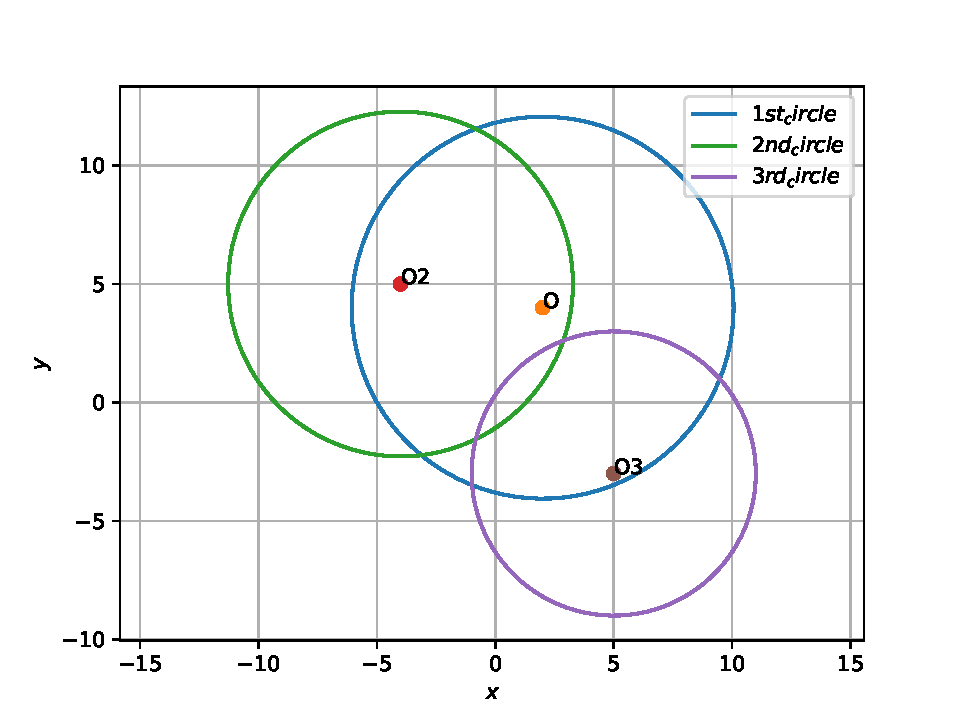
\includegraphics[width=\columnwidth]{./solutions/5/figs/circle/q18abc.eps}
	\caption{Circle of Q.4.2.5}
	\label{fig:4.2.5_qoec}	
	\end{figure}
\end{comment}
\item See Fig. \ref{fig:4.2.5_qoed}.
\begin{align}
\vec{O} = \frac{1}{4}\myvec{1\\0}, r = \frac{1}{4}
\end{align}
\begin{align} 
2\vec{x^Tx} - \myvec{1\\0}\vec{x} = 0
\end{align}
	\begin{figure}[!ht]
	\centering
	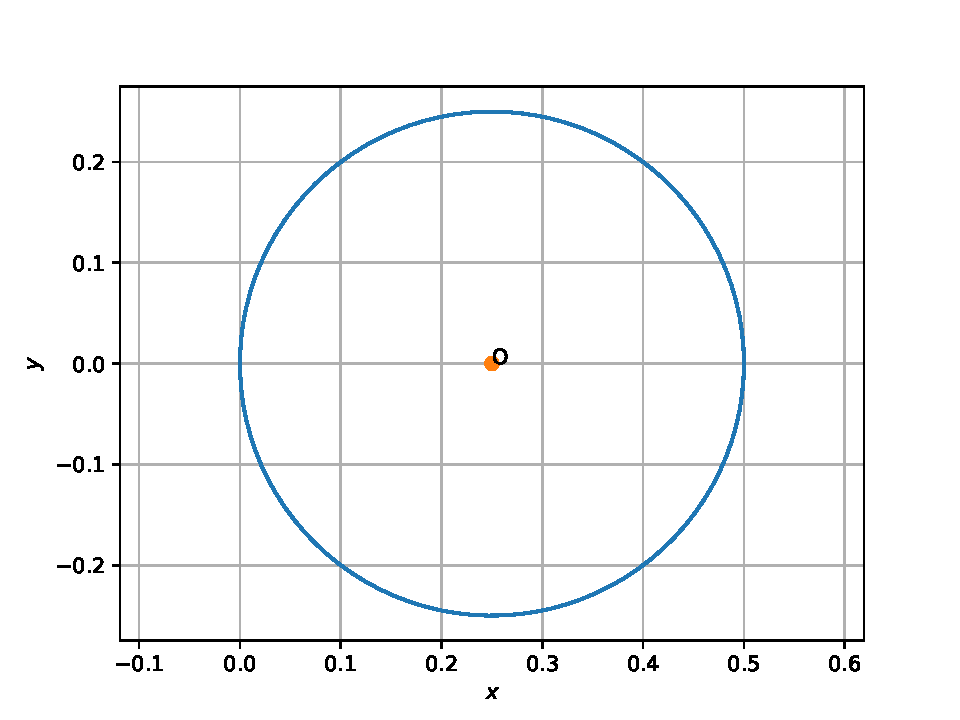
\includegraphics[width=\columnwidth]{./solutions/5/figs/circle/q18d.eps}
	\caption{}
	\label{fig:4.2.5_qoed}	
	\end{figure}



\end{enumerate}
